\scanpage{127}

% archive foliation: 126

\[
\deleted{(0,1)\to\infty}\quad (0,1)\to\unsure{\infty}\qquad (\infty,\tfrac12)\to0
\]
\[
\deleted{\frac{\unsure{az+b}\,(\unsure{c+d})z}{cz+d}}\quad\deleted{\unsure{az+d}}
\qquad z\mapsto\frac{\unsure{az|z}}{cz+(\unsure{d|1}-c)}
\]
\[
z\longrightarrow\frac{z\deleted{\unsure{+c-1}}}{cz+(1-c)}
\qquad\frac{z}{cz+(1-\unsure{z|c})}:\bigl(\frac{cz}{cz+1-c}+
\]

\figure{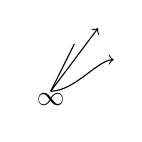
\begin{tikzpicture}[x=1cm,y=1cm]
\node at (0,0){$\uline{\infty}$};\draw[->](0,.1)--(.6,.9);\draw(0,.1)--(.3,.7);\draw[->](0,.1)..controls(.3,.1)and(.6,.5)..(.8,.5);
\end{tikzpicture}}

\figure{\begin{tikzpicture}[x=1cm,y=1cm]
\draw(0,0)ellipse(.85 and 1.25);\draw(.1,1.25)..controls(1.1,1.2)and(1.05,-1.2)..(.15,-1.25);
\draw(-.15,1.2)..controls(-.55,.75)and(-.5,.3)..(-.5,.15);\draw(-.5,-.3)..controls(-.5,-.85)and(-.2,-1.15)..(-.1,-1.25);
\fill(-.15,1.2)circle(.05);\fill(-.5,.15)circle(.035);\draw(-.1,-1.25)circle(.05);
\node[above]at(-.15,1.2){$0$};\node[below]at(-.1,-1.25){$1$};\node[left]at(-.5,.15){$\infty$};\node at(.55,.3){$\tfrac12$};
\end{tikzpicture}}

\figure{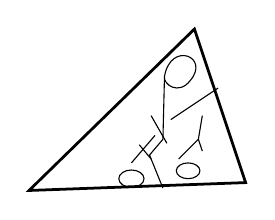
\begin{tikzpicture}[x=1cm,y=1cm]
\draw[line width=1pt](0,0)--(2.1,2.05)--(2.75,.1)--cycle;
\draw(1.7,.03)--(1.53,.45)--(1.7,.65)--(1.72,1.45)..controls(1.8,1.9)and(2.3,1.7)..(2.05,1.4)..controls(1.9,1.2)and(1.7,1.35)..(1.72,1.45);
\draw(1.3,.15)ellipse(.16 and .11);\draw(1.3,.35)--(1.6,.7);\draw(1.4,.58)--(1.55,.4);\draw(1.55,.95)--(1.75,.6);
\draw(2.02,.25)ellipse(.15 and .1);\draw(1.9,.4)--(2.15,.65)--(2.2,.95);\draw(2.15,.65)--(2.2,.5);\draw(1.8,.9)--(2.4,1.3);
\end{tikzpicture}}

\figure{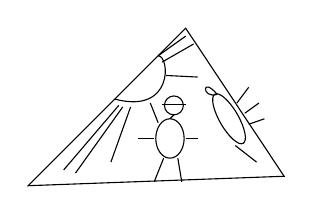
\begin{tikzpicture}[x=1cm,y=1cm]
\draw(0,0)--(2,2)--(3.25,.12)--cycle;
\draw(1.1,1.1)..controls(1.85,.9)and(1.8,1.65)..(1.65,1.65);
\draw(1.65,1.65)--(2,1.9);\draw(1.7,1.57)--(2.1,1.8);\draw(1.75,1.4)--(2.15,1.38);\draw(1.55,1.05)--(1.65,.8);
\draw(1.15,1.02)--(.45,.2);\draw(1.2,1)--(.6,.16);\draw(1.3,1)--(1.05,.3);
\draw(1.8,.6)ellipse(.18 and .25);\draw(1.85,1.02)circle(.12);\draw(1.8,.85)--(1.85,.9);\draw(1.72,.35)--(1.6,.05);\draw(1.9,.35)--(1.95,.05);\draw(1.6,.6)--(1.4,.6);\draw(2,.6)--(2.15,.6);\draw(1.7,1.03)--(2,1.03);
\draw[rotate around={30:(2.55,.85)}](2.55,.85)ellipse(.12 and .36);\draw(2.4,1.16)..controls(2.2,1.4)and(2.2,1.1)..(2.4,1.16);\draw(2.63,.51)--(2.9,.3);\draw(2.65,1.05)--(2.8,1.25);\draw(2.75,.92)--(2.93,1.05);\draw(2.8,.78)--(3,.85);
\end{tikzpicture}}

\[
\begin{pmatrix}1&0\\c&1-c\end{pmatrix}
\begin{pmatrix}1&\unsure{0}\\c&1-c\end{pmatrix}
\quad\begin{pmatrix}1&0\\2c-c^2&(1-c)^2\end{pmatrix}
\]
\[
(1-c)^2=1\qquad\deleted{\unsure{c}}\qquad c-1=\pm1\qquad c=0\text{ ou }2
\]

\figure{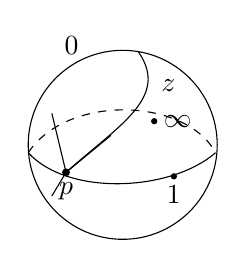
\begin{tikzpicture}[x=1cm,y=1cm]
\draw(0,0)circle(1.2);\draw(-1.2,-.1)..controls(-.7,-.65)and(.6,-.6)..(1.18,-.1);\draw[dashed](-1.2,-.1)..controls(-.7,.65)and(.8,.6)..(1.18,-.1);
\draw(.2,1.18)..controls(.6,.6)and(-.05,.25)..(-.72,-.35);\draw(-.9,.4)--(-.72,-.35)--(-.15,.12);\draw(-.9,-.65)--(-.72,-.35);
\fill(-.72,-.35)circle(.05);\fill(.65,-.4)circle(.04);\fill(.4,.3)circle(.04);\node[above]at(-.65,1.02){$0$};\node[below]at(-.72,-.35){$p$};\node[below]at(.65,-.4){$1$};\node[right]at(.4,.3){$\infty$};\node at(.58,.75){$z$};
\end{tikzpicture}}

\figure{
\begin{tikzpicture}[x=1cm,y=1cm]
\draw(-1.1,.7)..controls(-1.6,.55)and(-1.6,.4)..(-1.1,.45)--(.6,.55)..controls(1.6,.7)and(1.4,.8)..(.6,.8);
\draw(-1.1,.6)--(-1.1,1.1)..controls(-1.1,1.7)and(0,1.85)..(0,1.1)--(.05,.75)--(.25,.75);
\draw(-.85,.4)--(-.88,.05)--(-1,.0)--(-.75,-.03)--(-.68,-.13)--(-.75,-.2)--(-.55,-.24)--(-.6,-.34)--(-.43,-.4)--(-.43,-.55);
\draw(-.5,.35)--(.25,.45)--(.08,-.35)..controls(.6,.0)and(.9,.1)..(1.3,.15);
\draw(1.35,.1)..controls(1.8,.0)and(2,-.5)..(1.9,-.7);\draw(1.3,.15)--(.95,-.7);\draw(-.45,-.7)..controls(-.9,-1.2)and(-.2,-1.8)..(-.2,-1.8);\draw(.8,-1.2)--(2,-.9);
\draw(-.62,.3)--(-.5,.0)--(-.4,.2)--(-.65,.25)--(-.45,.05);
\end{tikzpicture}}

\figure{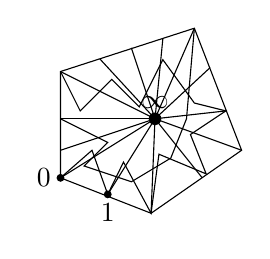
\begin{tikzpicture}[x=1cm,y=1cm]
\coordinate(O)at(0,0);\draw(-1.2,-.75)--(-1.2,.6)--(.5,1.15)--(1.1,-.4)--(-.05,-1.2)--cycle;
\foreach \p in {(-1.2,-.75),(-1.2,-.4),(-1.2,0),(-1.2,.6),(-.7,.76),(-.3,.9),(.1,1.02),(.5,1.15),(.7,.65),(.9,.1),(1.1,-.4),(.6,-.75),(-.05,-1.2),(-.6,-.96)}{\draw(O)--\p;}
\draw(-1.2,.6)--(-.95,.1)--(-.55,.5)--(-.2,.15)--(.1,.75)--(.5,.2)--(.9,.1)--(.45,-.2)--(.65,-.7)--(.05,-.45)--(-.05,-1.2)--(-.4,-.55)--(-.6,-.96)--(-.8,-.4)--(-1.2,-.75);
\draw(-1.2,0)--(-.6,-.3)--(-.9,-.6)--(-.3,-.8)--(.2,-.5)--(.4,0)--(.5,1.15);\fill(O)circle(.08);
\fill(-1.2,-.75)circle(.05);\fill(-.6,-.96)circle(.05);\node[left]at(-1.2,-.75){$0$};\node[below]at(-.6,-.96){$1$};\node[above]at(O){$\unsure{\infty}$};
\end{tikzpicture}}

\[
\frac{z}{2z-1}=\frac{1}{2-\tfrac1{\unsure{2|z}}}\qquad
z\unsure{=|\mathrel{,}}\frac{z}{2z-1}\qquad
\deleted{2}z^2-\deleted{2}z=0\qquad z=0\text{ ou }1
\]
\[
g\ \underbrace{0,1,\infty}\longrightarrow0\qquad
(0,\deleted{1},\infty)\to(0,\infty)
\]
\[
\deleted{\unsure{m}\;\;0,1}\quad1\to(0,\infty)\qquad\uuline{\text{ou}}\quad1
\]

\figure{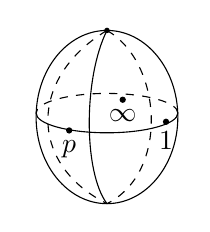
\begin{tikzpicture}[x=1cm,y=1cm]
\draw(0,0)ellipse(.9 and 1.1);\draw(0,1.1)..controls(-.3,.5)and(-.3,-.7)..(0,-1.1);
\draw(-.9,.05)arc(180:360:.9 and .25);\draw[dashed](.9,.05)arc(0:180:.9 and .25);
\draw[dashed](0,1.1)..controls(-1,.5)and(-1,-.6)..(0,-1.1);\draw[dashed](0,1.1)..controls(.7,.7)and(.8,-.7)..(0,-1.1);
\fill(0,1.1)circle(.035);\fill(-.48,-.17)circle(.04);\fill(.2,.22)circle(.04);\fill(.75,-.06)circle(.04);
\node[below]at(-.48,-.17){$p$};\node[below]at(.2,.22){$\infty$};\node[below]at(.75,-.06){$1$};
\end{tikzpicture}}

\figure{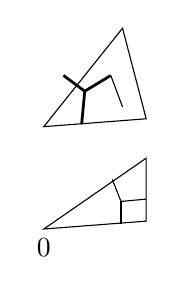
\begin{tikzpicture}[x=1cm,y=1cm]
\draw(0,0)--(1.3,.1)--(1,1.25)--cycle;\draw[line width=1pt](.85,.65)--(.52,.45)--(.25,.65);\draw[line width=1pt](.52,.45)--(.48,.03);\draw(1,.25)--(.85,.65);
\begin{scope}[yshift=-1.3cm]\draw(0,0)--(1.3,.1)--(1.3,.9)--cycle;\draw(1.3,.38)--(.98,.35)--(.87,.63);\draw(.98,.35)--(.98,.06);\node[below]at(0,0){$0$};\end{scope}
\end{tikzpicture}}

\[(0,1,\infty)\longrightarrow(0,1,\infty)\]
Si \deleted{\unsure{$s$ est $0,1,\infty$}}\inserted{$s=0,1,\infty$} \unsure{l'envoie en $1$}\par
\unsure{Il faut $f$ non ramifiée en $s$}\qquad $g$

\figure{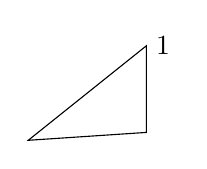
\begin{tikzpicture}[x=1cm,y=1cm]
\draw(0,0)--(1.5,.1)--(1.5,1.2)--cycle;\node[right]at(1.5,1.2){$1$};
\end{tikzpicture}}

\figure{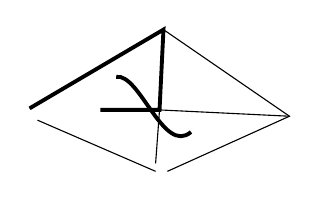
\begin{tikzpicture}[x=1cm,y=1cm]
\draw(-1.5,0)--(.2,1)--(1.8,-.1)--(.25,-.8);\draw(-1.4,-.15)--(.1,-.8);\draw[line width=1.4pt](-1.5,0)--(.2,1)--(.15,-.02)--(-.6,-.02);\draw(.15,-.02)--(.1,-.7);\draw(.15,-.02)--(1.8,-.1);
\draw[line width=1.4pt](-.4,.4)..controls(-.1,.45)and(.2,-.6)..(.55,-.3);
\end{tikzpicture}}

\figure{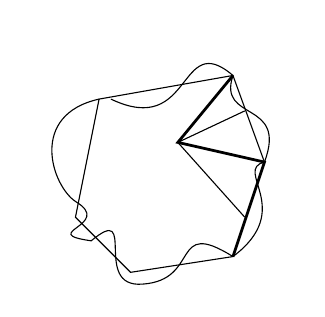
\begin{tikzpicture}[x=1cm,y=1cm]
\draw(-1,-.5)--(-.7,1)--(1,1.3)--(1.4,.2)--(1,-1)--(-.3,-1.2)--cycle;
\draw[line width=1pt](1,1.3)--(.3,.45)--(1.4,.2)--(1,-1);\draw(.3,.45)--(1.15,.85);\draw(.3,.45)--(1.15,-.5);
\draw(-.7,1)..controls(-1.6,.8)and(-1.3,-.1)..(-1,-.3)..controls(-.5,-.6)and(-1.5,-.7)..(-.8,-.8)..controls(-.2,-.3)and(-.8,-1.4)..(-.15,-1.35)..controls(.6,-1.3)and(.2,-.5)..(1,-1);
\draw(-.55,1)..controls(.5,.5)and(.3,1.9)..(1,1.3)..controls(.8,.7)and(1.7,1)..(1.4,.2)..controls(1,.1)and(1.8,-.4)..(1,-1);
\end{tikzpicture}}

\[f(z)\in[0,1]\qquad f(z)-\tfrac12\qquad (2f(z)-1)^2\]

\figure{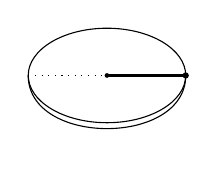
\begin{tikzpicture}[x=1cm,y=1cm]
\draw(0,0)ellipse(1 and .6);\draw(-1,0)..controls(-1,-.9)and(1,-.9)..(1,0);\draw[dotted](-1,0)--(0,0);\draw[line width=1pt](0,0)--(1,0);\fill(0,0)circle(.03);\fill(1,0)circle(.04);
\end{tikzpicture}}

\figure{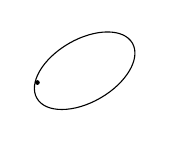
\begin{tikzpicture}[x=1cm,y=1cm]
\draw[rotate=30](0,0)ellipse(.7 and .4);\fill(-.6,-.15)circle(.03);
\end{tikzpicture}}

\figure{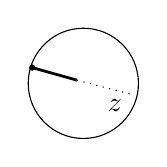
\begin{tikzpicture}[x=1cm,y=1cm]
\draw(0,0)circle(.7);\draw[line width=1pt](-.65,.2)--(-.08,.04);\draw[dotted](-.08,.04)--(.65,-.15);\fill(-.65,.2)circle(.04);\node at(.4,-.28){$z$};
\end{tikzpicture}}

\figure{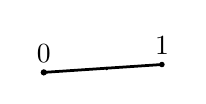
\begin{tikzpicture}[x=1cm,y=1cm]
\draw[line width=1pt](0,0)--(1.5,.1);\fill(0,0)circle(.04);\fill(1.5,.1)circle(.035);\fill(.8,.05)circle(.025);\node[above]at(0,0){$0$};\node[above]at(1.5,.1){$1$};
\end{tikzpicture}}

\figure{\begin{tikzpicture}[x=1cm,y=1cm]
\draw(-.7,0)--(.7,0);\draw(-.15,0)circle(.04);
\end{tikzpicture}}

\figure{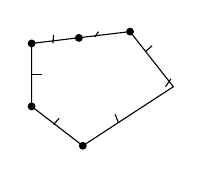
\begin{tikzpicture}[x=1cm,y=1cm]
\draw(0,0)--(0,.8)--(1.25,.95)--(1.8,.25)--(.65,-.5)--cycle;
\foreach \p in {(0,0),(0,.8),(.6,.87),(1.25,.95),(.65,-.5)}{\fill\p circle(.05);}
\draw(.27,.8)--(.28,.91);\draw(.8,.88)--(.85,.95);\draw(1.45,.7)--(1.53,.77);\draw(1.7,.25)--(1.77,.35);\draw(1.1,-.2)--(1.06,-.1);\draw(.28,-.23)--(.35,-.15);\draw(0,.4)--(.13,.4);
\end{tikzpicture}}

\figure{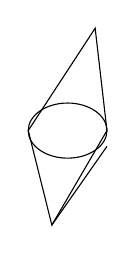
\begin{tikzpicture}[x=1cm,y=1cm]
\draw(0,0)ellipse(.5 and .35);\draw(-.5,0)--(.35,1.3)--(.5,0)--(-.2,-1.2)--cycle;\draw[thin](.5,-.2)--(-.2,-1.2);
\end{tikzpicture}}

\figure{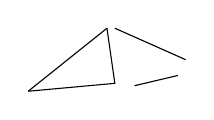
\begin{tikzpicture}[x=1cm,y=1cm]
\draw(-1,0)--(.1,.1)--(0,.8);\draw(.1,.8)--(1,.4);\draw(.35,.07)--(.9,.2);\draw[thin](-1,0)--(0,.8);
\end{tikzpicture}}

\[
g(z)=(2f(z)-1)^2\qquad(z-\tfrac12)^2\in[0,1]
\]
\[
\deleted{\unsure{z-\tfrac z2}}\qquad z\in[0,1]\quad\Updownarrow\quad
\deleted{2(z-\tfrac12)\in[\unsure{+}}\]
\[\deleted{g(z)=0\quad\Longrightarrow\quad f(z)=}\]
\[
\begin{array}{ll}g(z)=0&f(z)=\tfrac12\\g(z)=1&f(z)=0,1\end{array}
\qquad2z-1\in(-1,+1)\qquad(2z-1)^2\in[0,1]
\]
